\subsection{Local News and Local Terror}
Global terrorism does not correlate in a large context with local news, as the previous section showed (\textbf{Sicherstellen!!!!!}).
This section aimed to examine the hypothesis that (at least) local terror acts and local news about terror correlate.
For this we used the news articles provided from the \textit{zeit.de}-API,
so the considered terror attacks cover Germany.

To get the needed information from Zeit, we filtered the articles by location. \\
However, while the Zeit tags every article with the country it is related to if the country isn't Germany
(e.g. it uses both \textit{Rom} and \textit{Italien} if the article is about Rome),
it doesn't do that with articles related to locations in Germany.
Instead it only uses the city related to the article, e.g. \textit{Berlin}.
Therefore we used DBpedia's SPARQL-Endpoint to ask if the locations mentioned in the keywords of an article are a cities in Germany.

It was easy to get the relevant information from the GTD,
because every terror attack is tagged with the related country.
We used both the number of attacks and the number of casulties
in our research to find out if the seriousness of the attack effects the news.

The following images show the relativ number of articles in a month that deal with terrorism.
We use relative numbers,
because the absolute number of articles written per month in the zeit.de-database increased over time
(see \autoref{fig:zeit_total_number_of_articles} in the appendix).
We keep in mind that the number of articles between February 2006 and June 2008 drastically decreased.
With relative numbers we get the basic coverage of terrorism in the Zeit.
\begin{figure}[h]
  \centering
  \begin{subfigure}{1\textwidth}
    \centering
    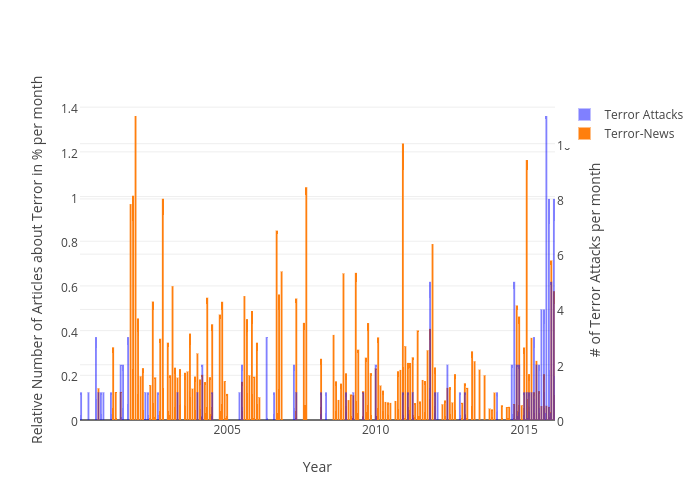
\includegraphics[width=.8\textwidth]{images/zeit/german_attacks}
    \caption{Terrorism-News and Number of Terrorism Attack (including Attempts)}
    \label{fig:zeit_terrorism_germany_attacks}
  \end{subfigure}
  \begin{subfigure}{1\textwidth}
    \centering
    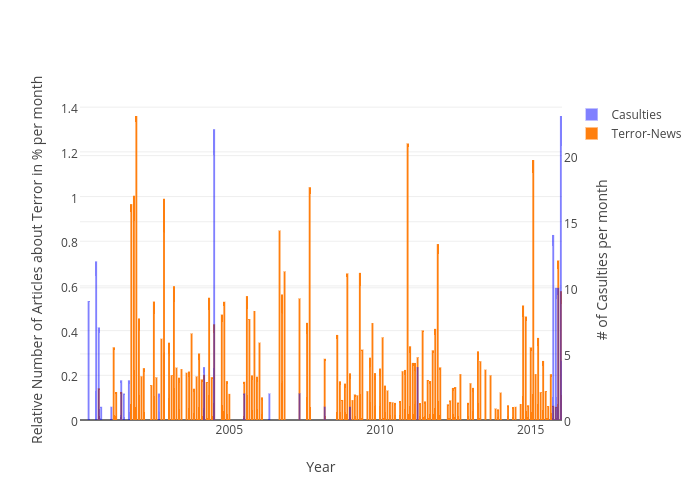
\includegraphics[width=.8\textwidth]{images/zeit/german_casulties}
    \caption{Terrorism-News and Number of Casulties (Injured + Killed)}
    \label{fig:zeit_terrorism_germany_casulties}
  \end{subfigure}
  \caption{Terrorism in Germany and News about Terrorism between 2000-2015}
  \label{fig:zeit_terrorism_germany}
\end{figure}
Both graphics in \autoref{fig:zeit_terrorism_germany} show, that the news in the Zeit doesn't correlate in a large scale.
While there are many terror-attacks (see \autoref{fig:zeit_terrorism_germany_attacks}) in the beginning of the century and even more at the end of 2015,
the Zeit published more news between end of 2001 to mid 2004 and between mid 2008 to end of 2011.
The first period of high frequency articles can be explained by the aftermath of 9/11 attacks,
dealing with, for example, security concerns that are related to Germany, too.

This shows that local news do not only report about terror when there are local incidents.
So we went further and also considered that local newspapers tend to cover not only local news,
but also news of their allies and reflect their situation onto themself.
Therefore we also included western countries in our research, i.e. countries in Western Europe and North America.
Similar to the filter-process to find articles related to Germany,
we used DBpedia to find out which countries are located in Western Europe and North America.
The process for GTD was very straight forward again,
as each recorded attack is also labeled with a region,
which include Western \textit{Europe} and \textit{North America}.

\begin{figure}[h]
  \centering
  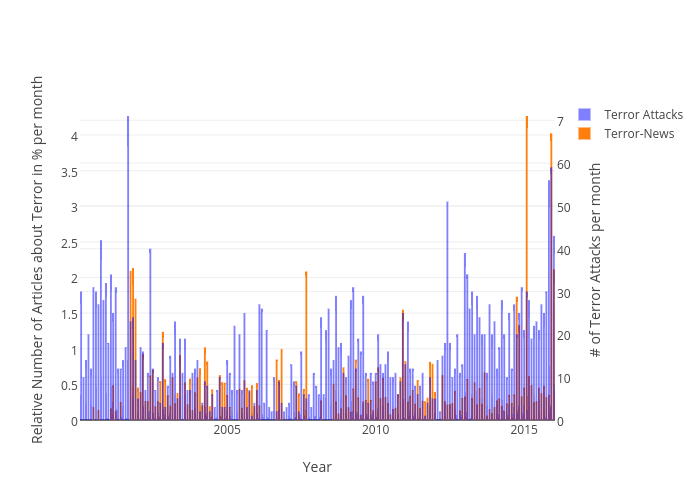
\includegraphics[width=.8\textwidth]{images/zeit/western_attacks}
  \caption{Terrorism-News and Number of Terrorism Attack (including Attempts)}
  \label{fig:zeit_terrorism_western_attacks}
\end{figure}
\autoref{fig:zeit_terrorism_western_attacks} shows the results of the above mentioned process.
Both datasets,
the number of terror attacks and the relative number of Articles about Terrorism,
are grouped into months again.
The two highes peaks with 4.2\% (January 2015) and 4\% (November 2015) of articles related to terrorism
are about the terror attacks in France (\textit{Charlie Hebdo shooting} respectively the \textit{Paris attacks})

\begin{figure}[h]
 \centering
 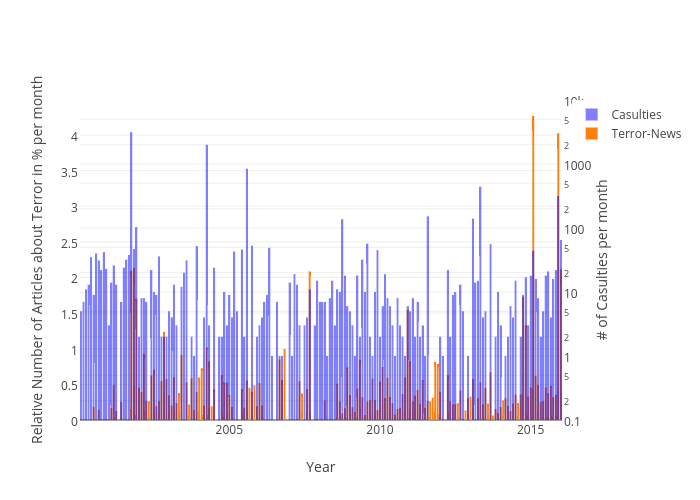
\includegraphics[width=.8\textwidth]{images/zeit/western_casulties}
 \caption{Terrorism-News and Number of Casulties (Injured + Killed)}
 \label{fig:zeit_terrorism_western_casulties}
\end{figure}
Here we look at the casulties instead of the number of attacks.
It is reasonable to believe that more articles about terrorism are published when the casulty-count reaches a certain threshold,
but higher casulties do not mean more more articles, we used a logarithmic scale for the number of casulties.
